\documentclass[twoside]{book}

% Packages required by doxygen
\usepackage{fixltx2e}
\usepackage{calc}
\usepackage{doxygen}
\usepackage[export]{adjustbox} % also loads graphicx
\usepackage{graphicx}
\usepackage[utf8]{inputenc}
\usepackage{makeidx}
\usepackage{multicol}
\usepackage{multirow}
\PassOptionsToPackage{warn}{textcomp}
\usepackage{textcomp}
\usepackage[nointegrals]{wasysym}
\usepackage[table]{xcolor}

% NLS support packages
\usepackage[spanish]{babel}
% Font selection
\usepackage[T1]{fontenc}
\usepackage[scaled=.90]{helvet}
\usepackage{courier}
\usepackage{amssymb}
\usepackage{sectsty}
\renewcommand{\familydefault}{\sfdefault}
\allsectionsfont{%
  \fontseries{bc}\selectfont%
  \color{darkgray}%
}
\renewcommand{\DoxyLabelFont}{%
  \fontseries{bc}\selectfont%
  \color{darkgray}%
}
\newcommand{\+}{\discretionary{\mbox{\scriptsize$\hookleftarrow$}}{}{}}

% Page & text layout
\usepackage{geometry}
\geometry{%
  a4paper,%
  top=2.5cm,%
  bottom=2.5cm,%
  left=2.5cm,%
  right=2.5cm%
}
\tolerance=750
\hfuzz=15pt
\hbadness=750
\setlength{\emergencystretch}{15pt}
\setlength{\parindent}{0cm}
\setlength{\parskip}{3ex plus 2ex minus 2ex}
\makeatletter
\renewcommand{\paragraph}{%
  \@startsection{paragraph}{4}{0ex}{-1.0ex}{1.0ex}{%
    \normalfont\normalsize\bfseries\SS@parafont%
  }%
}
\renewcommand{\subparagraph}{%
  \@startsection{subparagraph}{5}{0ex}{-1.0ex}{1.0ex}{%
    \normalfont\normalsize\bfseries\SS@subparafont%
  }%
}
\makeatother

% Headers & footers
\usepackage{fancyhdr}
\pagestyle{fancyplain}
\fancyhead[LE]{\fancyplain{}{\bfseries\thepage}}
\fancyhead[CE]{\fancyplain{}{}}
\fancyhead[RE]{\fancyplain{}{\bfseries\leftmark}}
\fancyhead[LO]{\fancyplain{}{\bfseries\rightmark}}
\fancyhead[CO]{\fancyplain{}{}}
\fancyhead[RO]{\fancyplain{}{\bfseries\thepage}}
\fancyfoot[LE]{\fancyplain{}{}}
\fancyfoot[CE]{\fancyplain{}{}}
\fancyfoot[RE]{\fancyplain{}{\bfseries\scriptsize Generado por Doxygen }}
\fancyfoot[LO]{\fancyplain{}{\bfseries\scriptsize Generado por Doxygen }}
\fancyfoot[CO]{\fancyplain{}{}}
\fancyfoot[RO]{\fancyplain{}{}}
\renewcommand{\footrulewidth}{0.4pt}
\renewcommand{\chaptermark}[1]{%
  \markboth{#1}{}%
}
\renewcommand{\sectionmark}[1]{%
  \markright{\thesection\ #1}%
}

% Indices & bibliography
\usepackage{natbib}
\usepackage[titles]{tocloft}
\setcounter{tocdepth}{3}
\setcounter{secnumdepth}{5}
\makeindex

% Hyperlinks (required, but should be loaded last)
\usepackage{ifpdf}
\ifpdf
  \usepackage[pdftex,pagebackref=true]{hyperref}
\else
  \usepackage[ps2pdf,pagebackref=true]{hyperref}
\fi
\hypersetup{%
  colorlinks=true,%
  linkcolor=blue,%
  citecolor=blue,%
  unicode%
}

% Custom commands
\newcommand{\clearemptydoublepage}{%
  \newpage{\pagestyle{empty}\cleardoublepage}%
}

\usepackage{caption}
\captionsetup{labelsep=space,justification=centering,font={bf},singlelinecheck=off,skip=4pt,position=top}

%===== C O N T E N T S =====

\begin{document}

% Titlepage & ToC
\hypersetup{pageanchor=false,
             bookmarksnumbered=true,
             pdfencoding=unicode
            }
\pagenumbering{alph}
\begin{titlepage}
\vspace*{7cm}
\begin{center}%
{\Large Plantilla\+\_\+5to \\[1ex]\large 1.\+0 }\\
\vspace*{1cm}
{\large Generado por Doxygen 1.8.13}\\
\end{center}
\end{titlepage}
\clearemptydoublepage
\pagenumbering{roman}
\tableofcontents
\clearemptydoublepage
\pagenumbering{arabic}
\hypersetup{pageanchor=true}

%--- Begin generated contents ---
\chapter{Indice de archivos}
\section{Lista de archivos}
Lista de todos los archivos con descripciones breves\+:\begin{DoxyCompactList}
\item\contentsline{section}{\hyperlink{confbits_8h}{confbits.\+h} }{\pageref{confbits_8h}}{}
\item\contentsline{section}{\hyperlink{FW__InitKit_8c}{F\+W\+\_\+\+Init\+Kit.\+c} }{\pageref{FW__InitKit_8c}}{}
\item\contentsline{section}{\hyperlink{FW__InitKit_8h}{F\+W\+\_\+\+Init\+Kit.\+h} }{\pageref{FW__InitKit_8h}}{}
\item\contentsline{section}{\hyperlink{Interrupciones_8c}{Interrupciones.\+c} }{\pageref{Interrupciones_8c}}{}
\item\contentsline{section}{\hyperlink{lemos_8c}{lemos.\+c} }{\pageref{lemos_8c}}{}
\item\contentsline{section}{\hyperlink{lemos_8h}{lemos.\+h} }{\pageref{lemos_8h}}{}
\item\contentsline{section}{\hyperlink{lopez_8c}{lopez.\+c} }{\pageref{lopez_8c}}{}
\item\contentsline{section}{\hyperlink{main_8c}{main.\+c} }{\pageref{main_8c}}{}
\end{DoxyCompactList}

\chapter{Documentación de archivos}
\hypertarget{confbits_8h}{}\section{Referencia del Archivo confbits.\+h}
\label{confbits_8h}\index{confbits.\+h@{confbits.\+h}}
Gráfico de los archivos que directa o indirectamente incluyen a este archivo\+:
\nopagebreak
\begin{figure}[H]
\begin{center}
\leavevmode
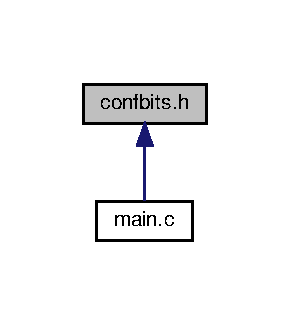
\includegraphics[width=139pt]{db/d61/confbits_8h__dep__incl}
\end{center}
\end{figure}

\input{d6/d67/FW__InitKit_8c}
\input{d5/dee/FW__InitKit_8h}
\input{db/df9/FW__Timer_8c}
\input{df/dcc/FW__Timer_8h}
\hypertarget{Interrupciones_8c}{}\section{Referencia del Archivo Interrupciones.\+c}
\label{Interrupciones_8c}\index{Interrupciones.\+c@{Interrupciones.\+c}}
{\ttfamily \#include $<$xc.\+h$>$}\newline
{\ttfamily \#include \char`\"{}lemos.\+h\char`\"{}}\newline
Dependencia gráfica adjunta para Interrupciones.\+c\+:\nopagebreak
\begin{figure}[H]
\begin{center}
\leavevmode
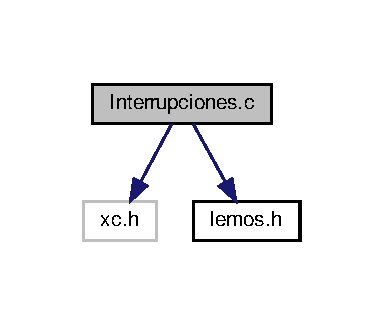
\includegraphics[width=184pt]{dc/dc1/Interrupciones_8c__incl}
\end{center}
\end{figure}

\hypertarget{lemos_8c}{}\section{Referencia del Archivo lemos.\+c}
\label{lemos_8c}\index{lemos.\+c@{lemos.\+c}}
{\ttfamily \#include $<$xc.\+h$>$}\newline
{\ttfamily \#include \char`\"{}Ap\+\_\+ini.\+h\char`\"{}}\newline
{\ttfamily \#include \char`\"{}lemos.\+h\char`\"{}}\newline
Dependencia gráfica adjunta para lemos.\+c\+:\nopagebreak
\begin{figure}[H]
\begin{center}
\leavevmode
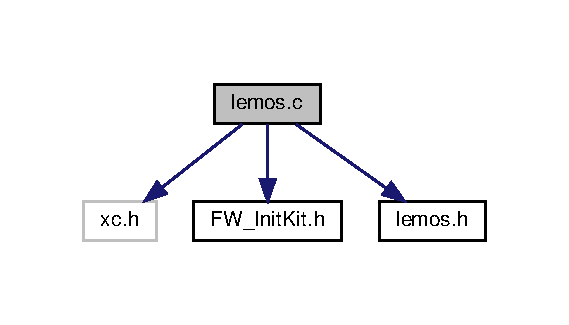
\includegraphics[width=255pt]{d3/d9f/lemos_8c__incl}
\end{center}
\end{figure}
\subsection*{Funciones}
\begin{DoxyCompactItemize}
\item 
void \hyperlink{lemos_8c_ae047d905d36b056a0cefa05604fceb1d}{leds} (unsigned int velocidad)
\item 
void \hyperlink{lemos_8c_a7a40b0fc89a60e6580ebc02dabdcc932}{Send\+\_\+\+Disp} (unsigned char Nro\+Disp, unsigned char Dato)
\item 
void \hyperlink{lemos_8c_a04efd902b97e8e6615ce019080aa7a4c}{Send\+\_\+4\+Disp} (unsigned char Umil, unsigned char Cent, unsigned char Dec, unsigned char Uni)
\item 
void \hyperlink{lemos_8c_a9d14fc429e90fdd19f4c3b06e12dba55}{tic\+\_\+timer0} (void)
\end{DoxyCompactItemize}


\subsection{Documentación de las funciones}
\mbox{\Hypertarget{lemos_8c_ae047d905d36b056a0cefa05604fceb1d}\label{lemos_8c_ae047d905d36b056a0cefa05604fceb1d}} 
\index{lemos.\+c@{lemos.\+c}!leds@{leds}}
\index{leds@{leds}!lemos.\+c@{lemos.\+c}}
\subsubsection{\texorpdfstring{leds()}{leds()}}
{\footnotesize\ttfamily void leds (\begin{DoxyParamCaption}\item[{unsigned int}]{velocidad }\end{DoxyParamCaption})}



Definición en la línea 12 del archivo lemos.\+c.

\mbox{\Hypertarget{lemos_8c_a04efd902b97e8e6615ce019080aa7a4c}\label{lemos_8c_a04efd902b97e8e6615ce019080aa7a4c}} 
\index{lemos.\+c@{lemos.\+c}!Send\+\_\+4\+Disp@{Send\+\_\+4\+Disp}}
\index{Send\+\_\+4\+Disp@{Send\+\_\+4\+Disp}!lemos.\+c@{lemos.\+c}}
\subsubsection{\texorpdfstring{Send\+\_\+4\+Disp()}{Send\_4Disp()}}
{\footnotesize\ttfamily void Send\+\_\+4\+Disp (\begin{DoxyParamCaption}\item[{unsigned char}]{Umil,  }\item[{unsigned char}]{Cent,  }\item[{unsigned char}]{Dec,  }\item[{unsigned char}]{Uni }\end{DoxyParamCaption})}



Definición en la línea 78 del archivo lemos.\+c.

\mbox{\Hypertarget{lemos_8c_a7a40b0fc89a60e6580ebc02dabdcc932}\label{lemos_8c_a7a40b0fc89a60e6580ebc02dabdcc932}} 
\index{lemos.\+c@{lemos.\+c}!Send\+\_\+\+Disp@{Send\+\_\+\+Disp}}
\index{Send\+\_\+\+Disp@{Send\+\_\+\+Disp}!lemos.\+c@{lemos.\+c}}
\subsubsection{\texorpdfstring{Send\+\_\+\+Disp()}{Send\_Disp()}}
{\footnotesize\ttfamily void Send\+\_\+\+Disp (\begin{DoxyParamCaption}\item[{unsigned char}]{Nro\+Disp,  }\item[{unsigned char}]{Dato }\end{DoxyParamCaption})}



Definición en la línea 47 del archivo lemos.\+c.

\mbox{\Hypertarget{lemos_8c_a9d14fc429e90fdd19f4c3b06e12dba55}\label{lemos_8c_a9d14fc429e90fdd19f4c3b06e12dba55}} 
\index{lemos.\+c@{lemos.\+c}!tic\+\_\+timer0@{tic\+\_\+timer0}}
\index{tic\+\_\+timer0@{tic\+\_\+timer0}!lemos.\+c@{lemos.\+c}}
\subsubsection{\texorpdfstring{tic\+\_\+timer0()}{tic\_timer0()}}
{\footnotesize\ttfamily void tic\+\_\+timer0 (\begin{DoxyParamCaption}\item[{void}]{ }\end{DoxyParamCaption})}



Definición en la línea 121 del archivo lemos.\+c.


\hypertarget{lemos_8h}{}\section{Referencia del Archivo lemos.\+h}
\label{lemos_8h}\index{lemos.\+h@{lemos.\+h}}
Gráfico de los archivos que directa o indirectamente incluyen a este archivo\+:
\nopagebreak
\begin{figure}[H]
\begin{center}
\leavevmode
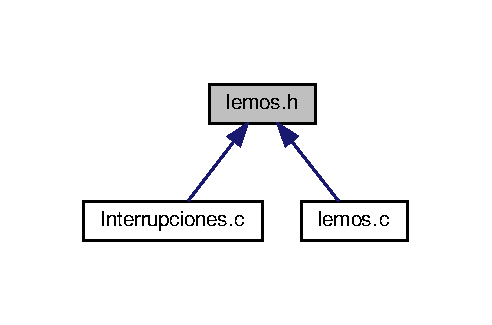
\includegraphics[width=236pt]{d5/d17/lemos_8h__dep__incl}
\end{center}
\end{figure}
\subsection*{defines}
\begin{DoxyCompactItemize}
\item 
\#define \hyperlink{lemos_8h_a23b9dfb70246e7331808b61afbc2641a}{include\+\_\+guard\+\_\+symbol}~\}
\item 
\#define \hyperlink{lemos_8h_a3c8594af1ba7b43bd07678516eee97ee}{L\+E\+M\+O\+S\+\_\+H}
\item 
\#define \hyperlink{lemos_8h_a5100621ffac89891837769883fc2c758}{M\+U\+X\+\_\+\+S\+ET}~4;
\item 
\#define \hyperlink{lemos_8h_a05a87a2b06b697c93c5439bf3e17a40f}{B\+O\+T\+\_\+\+R\+EL}~100;
\end{DoxyCompactItemize}
\subsection*{Funciones}
\begin{DoxyCompactItemize}
\item 
void \hyperlink{lemos_8h_a04efd902b97e8e6615ce019080aa7a4c}{Send\+\_\+4\+Disp} (unsigned char Umil, unsigned char Cent, unsigned char Dec, unsigned char Uni)
\item 
void \hyperlink{lemos_8h_ae047d905d36b056a0cefa05604fceb1d}{leds} (unsigned int velocidad)
\item 
void \hyperlink{lemos_8h_a9d14fc429e90fdd19f4c3b06e12dba55}{tic\+\_\+timer0} (void)
\end{DoxyCompactItemize}
\subsection*{Variables}
\begin{DoxyCompactItemize}
\item 
unsigned char \hyperlink{lemos_8h_a7475a5f89581dfb75e5d89d871ef793a}{mux\+\_\+tout}
\item 
unsigned char \hyperlink{lemos_8h_af41312e93852b1cf62bd17fff9a05871}{bot\+\_\+tout}
\item 
unsigned int \hyperlink{lemos_8h_a73ee79a6ecfafaa8a96a55ce82fd4506}{led\+\_\+tout}
\end{DoxyCompactItemize}


\subsection{Documentación de los \textquotesingle{}defines\textquotesingle{}}
\mbox{\Hypertarget{lemos_8h_a05a87a2b06b697c93c5439bf3e17a40f}\label{lemos_8h_a05a87a2b06b697c93c5439bf3e17a40f}} 
\index{lemos.\+h@{lemos.\+h}!B\+O\+T\+\_\+\+R\+EL@{B\+O\+T\+\_\+\+R\+EL}}
\index{B\+O\+T\+\_\+\+R\+EL@{B\+O\+T\+\_\+\+R\+EL}!lemos.\+h@{lemos.\+h}}
\subsubsection{\texorpdfstring{B\+O\+T\+\_\+\+R\+EL}{BOT\_REL}}
{\footnotesize\ttfamily \#define B\+O\+T\+\_\+\+R\+EL~100;}



Definición en la línea 61 del archivo lemos.\+h.

\mbox{\Hypertarget{lemos_8h_a23b9dfb70246e7331808b61afbc2641a}\label{lemos_8h_a23b9dfb70246e7331808b61afbc2641a}} 
\index{lemos.\+h@{lemos.\+h}!include\+\_\+guard\+\_\+symbol@{include\+\_\+guard\+\_\+symbol}}
\index{include\+\_\+guard\+\_\+symbol@{include\+\_\+guard\+\_\+symbol}!lemos.\+h@{lemos.\+h}}
\subsubsection{\texorpdfstring{include\+\_\+guard\+\_\+symbol}{include\_guard\_symbol}}
{\footnotesize\ttfamily \#define include\+\_\+guard\+\_\+symbol~\}}

\mbox{\Hypertarget{lemos_8h_a3c8594af1ba7b43bd07678516eee97ee}\label{lemos_8h_a3c8594af1ba7b43bd07678516eee97ee}} 
\index{lemos.\+h@{lemos.\+h}!L\+E\+M\+O\+S\+\_\+H@{L\+E\+M\+O\+S\+\_\+H}}
\index{L\+E\+M\+O\+S\+\_\+H@{L\+E\+M\+O\+S\+\_\+H}!lemos.\+h@{lemos.\+h}}
\subsubsection{\texorpdfstring{L\+E\+M\+O\+S\+\_\+H}{LEMOS\_H}}
{\footnotesize\ttfamily \#define L\+E\+M\+O\+S\+\_\+H}

\mbox{\Hypertarget{lemos_8h_a5100621ffac89891837769883fc2c758}\label{lemos_8h_a5100621ffac89891837769883fc2c758}} 
\index{lemos.\+h@{lemos.\+h}!M\+U\+X\+\_\+\+S\+ET@{M\+U\+X\+\_\+\+S\+ET}}
\index{M\+U\+X\+\_\+\+S\+ET@{M\+U\+X\+\_\+\+S\+ET}!lemos.\+h@{lemos.\+h}}
\subsubsection{\texorpdfstring{M\+U\+X\+\_\+\+S\+ET}{MUX\_SET}}
{\footnotesize\ttfamily \#define M\+U\+X\+\_\+\+S\+ET~4;}



Definición en la línea 60 del archivo lemos.\+h.



\subsection{Documentación de las funciones}
\mbox{\Hypertarget{lemos_8h_ae047d905d36b056a0cefa05604fceb1d}\label{lemos_8h_ae047d905d36b056a0cefa05604fceb1d}} 
\index{lemos.\+h@{lemos.\+h}!leds@{leds}}
\index{leds@{leds}!lemos.\+h@{lemos.\+h}}
\subsubsection{\texorpdfstring{leds()}{leds()}}
{\footnotesize\ttfamily void leds (\begin{DoxyParamCaption}\item[{unsigned int}]{velocidad }\end{DoxyParamCaption})}



Definición en la línea 12 del archivo lemos.\+c.

\mbox{\Hypertarget{lemos_8h_a04efd902b97e8e6615ce019080aa7a4c}\label{lemos_8h_a04efd902b97e8e6615ce019080aa7a4c}} 
\index{lemos.\+h@{lemos.\+h}!Send\+\_\+4\+Disp@{Send\+\_\+4\+Disp}}
\index{Send\+\_\+4\+Disp@{Send\+\_\+4\+Disp}!lemos.\+h@{lemos.\+h}}
\subsubsection{\texorpdfstring{Send\+\_\+4\+Disp()}{Send\_4Disp()}}
{\footnotesize\ttfamily void Send\+\_\+4\+Disp (\begin{DoxyParamCaption}\item[{unsigned char}]{Umil,  }\item[{unsigned char}]{Cent,  }\item[{unsigned char}]{Dec,  }\item[{unsigned char}]{Uni }\end{DoxyParamCaption})}



Definición en la línea 78 del archivo lemos.\+c.

\mbox{\Hypertarget{lemos_8h_a9d14fc429e90fdd19f4c3b06e12dba55}\label{lemos_8h_a9d14fc429e90fdd19f4c3b06e12dba55}} 
\index{lemos.\+h@{lemos.\+h}!tic\+\_\+timer0@{tic\+\_\+timer0}}
\index{tic\+\_\+timer0@{tic\+\_\+timer0}!lemos.\+h@{lemos.\+h}}
\subsubsection{\texorpdfstring{tic\+\_\+timer0()}{tic\_timer0()}}
{\footnotesize\ttfamily void tic\+\_\+timer0 (\begin{DoxyParamCaption}\item[{void}]{ }\end{DoxyParamCaption})}



Definición en la línea 121 del archivo lemos.\+c.



\subsection{Documentación de las variables}
\mbox{\Hypertarget{lemos_8h_af41312e93852b1cf62bd17fff9a05871}\label{lemos_8h_af41312e93852b1cf62bd17fff9a05871}} 
\index{lemos.\+h@{lemos.\+h}!bot\+\_\+tout@{bot\+\_\+tout}}
\index{bot\+\_\+tout@{bot\+\_\+tout}!lemos.\+h@{lemos.\+h}}
\subsubsection{\texorpdfstring{bot\+\_\+tout}{bot\_tout}}
{\footnotesize\ttfamily unsigned char bot\+\_\+tout}



Definición en la línea 57 del archivo lemos.\+h.

\mbox{\Hypertarget{lemos_8h_a73ee79a6ecfafaa8a96a55ce82fd4506}\label{lemos_8h_a73ee79a6ecfafaa8a96a55ce82fd4506}} 
\index{lemos.\+h@{lemos.\+h}!led\+\_\+tout@{led\+\_\+tout}}
\index{led\+\_\+tout@{led\+\_\+tout}!lemos.\+h@{lemos.\+h}}
\subsubsection{\texorpdfstring{led\+\_\+tout}{led\_tout}}
{\footnotesize\ttfamily unsigned int led\+\_\+tout}



Definición en la línea 58 del archivo lemos.\+h.

\mbox{\Hypertarget{lemos_8h_a7475a5f89581dfb75e5d89d871ef793a}\label{lemos_8h_a7475a5f89581dfb75e5d89d871ef793a}} 
\index{lemos.\+h@{lemos.\+h}!mux\+\_\+tout@{mux\+\_\+tout}}
\index{mux\+\_\+tout@{mux\+\_\+tout}!lemos.\+h@{lemos.\+h}}
\subsubsection{\texorpdfstring{mux\+\_\+tout}{mux\_tout}}
{\footnotesize\ttfamily unsigned char mux\+\_\+tout}



Definición en la línea 57 del archivo lemos.\+h.


\hypertarget{lopez_8c}{}\section{Referencia del Archivo lopez.\+c}
\label{lopez_8c}\index{lopez.\+c@{lopez.\+c}}

\hypertarget{main_8c}{}\section{Referencia del Archivo main.\+c}
\label{main_8c}\index{main.\+c@{main.\+c}}
{\ttfamily \#include $<$xc.\+h$>$}\newline
{\ttfamily \#include \char`\"{}confbits.\+h\char`\"{}}\newline
Dependencia gráfica adjunta para main.\+c\+:\nopagebreak
\begin{figure}[H]
\begin{center}
\leavevmode
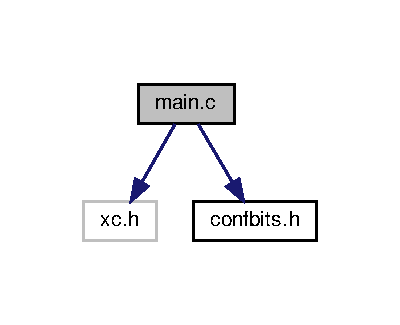
\includegraphics[width=192pt]{d4/d10/main_8c__incl}
\end{center}
\end{figure}
\subsection*{Funciones}
\begin{DoxyCompactItemize}
\item 
void \hyperlink{main_8c_a6288eba0f8e8ad3ab1544ad731eb7667}{main} (void)
\item 
void \hyperlink{main_8c_ae1d3159fc186c5f0bef6dd9a22c58859}{\+\_\+\+\_\+interrupt} ()
\end{DoxyCompactItemize}


\subsection{Documentación de las funciones}
\mbox{\Hypertarget{main_8c_ae1d3159fc186c5f0bef6dd9a22c58859}\label{main_8c_ae1d3159fc186c5f0bef6dd9a22c58859}} 
\index{main.\+c@{main.\+c}!\+\_\+\+\_\+interrupt@{\+\_\+\+\_\+interrupt}}
\index{\+\_\+\+\_\+interrupt@{\+\_\+\+\_\+interrupt}!main.\+c@{main.\+c}}
\subsubsection{\texorpdfstring{\+\_\+\+\_\+interrupt()}{\_\_interrupt()}}
{\footnotesize\ttfamily void \+\_\+\+\_\+interrupt (\begin{DoxyParamCaption}{ }\end{DoxyParamCaption})}



Definición en la línea 67 del archivo main.\+c.

\mbox{\Hypertarget{main_8c_a6288eba0f8e8ad3ab1544ad731eb7667}\label{main_8c_a6288eba0f8e8ad3ab1544ad731eb7667}} 
\index{main.\+c@{main.\+c}!main@{main}}
\index{main@{main}!main.\+c@{main.\+c}}
\subsubsection{\texorpdfstring{main()}{main()}}
{\footnotesize\ttfamily void main (\begin{DoxyParamCaption}\item[{void}]{ }\end{DoxyParamCaption})}



Definición en la línea 58 del archivo main.\+c.


%--- End generated contents ---

% Index
\backmatter
\newpage
\phantomsection
\clearemptydoublepage
\addcontentsline{toc}{chapter}{Índice}
\printindex

\end{document}
